\chapter*{Závěr} % SEM NESAHEJTE!
\addcontentsline{toc}{chapter}{Závěr} % SEM NESAHEJTE!
\markboth{Závěr}{Závěr}
V rámci projektu jsme provedli dvě měření. Při prvním měření bylo za cíl získat závislost ztrát na poloze dvou antén ve statickém prostředí pro úzkopásmový přenos. V našem případě proběhlo měření tak, že byla pevně umístěná vysílací anténa a zaznamenávali jsme hodnoty síly signálu v závislosti na vzdálenosti od vysílací antény. Jako lokaci měření jsme si zvolili městskou zástavbu a to konkrétně ulice Jugoslávských partyzánů a ulici Terronskou. Měření jsme tedy provedli dvakrát abychom měli lepší představu o problematice měření a mohli porovnat naměřené výsledky a diskutovat faktory, které výsledky mohly ovlivnit.
Hodnoty útlumu byly měřeny od 10 m do 350 m od vysílací antény za pomoci přenosného spektrálního analyzátoru. Vysílací anténa byla monopólová a uchycena na trojnožku. Měření probíhalo na frekvenci 1 GHz. 
Z dat vynesených do grafů lze vidět, že hodnoty naměřené v ulici Jugoslávských partyzánů jsou více dynamicky proměnlivé. To bylo způsobeno pohybem mnoha osob a vozidel v této rušné ulici. U průběhů naměřených v ulici Terronská jsou více patrné odrazy od statických okolních objektů v ulici. U obou měření je ale dobře viditelný trend celkového útlumu. Data odpovídají predikcím empirického modelu jak v grafu distribuční funkce, tak i v grafu normálového rozdělení hodnot. Vypočtený koeficient $n$ v prvním případě byl 4,70 a 3,81 v druhém případě. Tyto hodnoty dle tabulky odpovídají husté zástavbě.

Při druhém měření byl cíl zaznamenat časový průběh útlumu při statickém umístění obou antén ve třech případech a to při neovlivnění spoje, dynamické zastínění spoje a úplné zastínění spoje. 
Jako místo měření jsme zvolili vchod Technické menzy, kde se v době měření pohybovalo velké množství lidí. Antény byly umístěny na chodníku ve vzdálenosti 24 m a výšce 1,4 m pro vyšší pravděpodobnost zastínění. 
Díky umístení a času měření jsme však nebyli pořádně schopni změřit delší úsek dat pro nezastínený spoj. A tedy pro účel analýzy jsme spojili několik segmentů vzorků za sebe. Měření dynamického zastínění proběhlo bez problému. Měření úplného zastínění se ukázalo jako obtížnější, proto jsme se zapojili i my a pohybovali se mezi anténami. Z důvodu delší analýzy dat jsme v tomto případě vložili segment několikrát za sebe. 
Z vykreslení vzorků do grafu v čase můžeme dobře vidět jak se od sebe liší situace nezastíněného a dynamicky zastíněného spoje. U dynamicky zastíněného spoje je vidět mnohem více časových změn od pohybujících se osob a útlum je mnohem nižší.

\clearpage

\begin{figure}[h!]
    \centering
    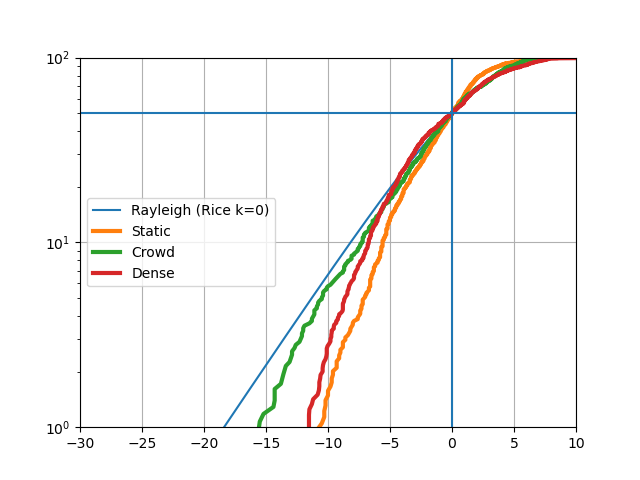
\includegraphics[,scale=0.85]{img/all_scenario.png}
    \caption{Porovnání výsledných distribučních funkcí}
    \label{fig:my_label}
\end{figure}

Z výsledků tohoto projektu jsme mohli dobře vidět, jak se síla přijímaného signálu mění v čase v závislosti na dynamičnosti okolí, a také jak je jeho útlum závislý na celkovém prostředí a vzdálenosti od vysílače. Také jsme se přesvědčili, jaké děje ovlivňují kvalitu spojení tak jako je tomu například u spoje mobilního telefonu s pozemním vysílačem ve městě. 